% Premier League Graph - arXiv preprint. Compile: pdflatex main && pdflatex main
\documentclass[11pt]{article}
\usepackage[T5,T1]{fontenc}
\usepackage[utf8]{inputenc}
\usepackage[vietnamese,english]{babel}
\usepackage{newtxtext,newtxmath}
\usepackage[letterpaper,margin=1in]{geometry}
\usepackage{microtype,graphicx,booktabs,multirow,array,tabularx,xcolor,enumitem,amsmath,fancyhdr,caption,float}
\usepackage[hidelinks]{hyperref}
\usepackage{tikz}
\usetikzlibrary{positioning,arrows.meta,calc,fit,backgrounds}

% ---------------- arXiv preprint look ----------------
\pagestyle{fancy}\fancyhf{}
\fancyhead[C]{\small\scshape A preprint -- \today}
\fancyfoot[C]{\thepage}
\renewcommand{\headrulewidth}{0pt}
\setlength{\parskip}{0.4em}\setlength{\parindent}{0pt}
\captionsetup{font=small,labelfont=bf}
\setlist{nosep,leftmargin=1.2em}
\newcommand{\vi}[1]{\foreignlanguage{vietnamese}{#1}}
\newcommand{\rel}[1]{\texttt{\detokenize{#1}}}
\newcommand{\hop}[1]{\texttt{\detokenize{#1}}}

\title{\vspace{-1.5em}\rule{\linewidth}{3pt}\\[0.6em]
\Large\bfseries BUILDING AND QUERYING A PREMIER LEAGUE SOCIAL NETWORK FROM VIETNAMESE AND ENGLISH NEWS WITH A 4B-PARAMETER LANGUAGE MODEL\\[0.4em]\rule{\linewidth}{1pt}}
\author{%
\small\begin{tabular}{c@{\hspace{2.2em}}c@{\hspace{2.2em}}c}
\textbf{\vi{Minh-Quân Lê}} & \textbf{\vi{Huyền-Mi Bùi}} & \textbf{\vi{Mai-Vũ Trần}}\\
\texttt{23020563@vnu.edu.vn} & \texttt{23020549@vnu.edu.vn} & \texttt{vutm@vnu.edu.vn}\\[0.3em]
\multicolumn{3}{c}{VNU University of Engineering and Technology, Xuan Thuy, Cau Giay, Hanoi, Vietnam}
\end{tabular}}
\date{}

\begin{document}
\maketitle
\thispagestyle{fancy}

\begin{abstract}
We build a knowledge graph of players, coaches, agents and clubs around the English Premier League from 6,158 Vietnamese and English news articles, and an application that answers multi-hop questions over it. Relations are extracted by Qwen3-4B, fine-tuned with LoRA on labels from a larger teacher model on two free T4 GPUs. Every person is linked to Wikidata, and an edge that has a single piece of evidence and is not confirmed by Wikidata is dropped. The resulting graph has 2,046 nodes and 4,924 evidence-backed edges of 12 relation types. Its estimated precision is 93\%, close to the 94.0\% of a graph extracted with Qwen3-14B, although the 4B model trails by 7--9 F1 points at the extraction step. The teammate network derived from career dates is a small world ($\sigma = 9.23$). Its Leiden communities follow clubs (NMI 0.62), and its 41-core contains all of the 20 highest-PageRank players. For question answering, the model plans a path over a typed catalogue of 29 hops instead of writing Cypher. Deterministic checks then inspect the plan, and the model re-plans with reasoning only when a check fires. On 100 held-out questions this answers 95\% correctly, against 89\% for three-vote self-consistency and 94\% for always-on reasoning, at a median of 1.8\,s per question. Self-consistency voting did not change a single answer, because the planner's mistakes are systematic. Data and code: \url{https://github.com/minquanle/premier-league-graph}.
\end{abstract}
\textbf{\textit{Keywords}}\enspace Knowledge graph $\cdot$ Relation extraction $\cdot$ Knowledge distillation $\cdot$ Social network analysis $\cdot$ GraphRAG $\cdot$ Small language models

% =====================================================================
\section{Introduction}
Football news is a dense record of social relations: who plays for whom, which coach was appointed or sacked, which pundit criticised which player, which agent represents whom. Vietnamese sports media cover the Premier League in great volume, yet this information stays locked in text. Knowledge graphs turn such text into a structure that supports network analysis and question answering, and large language models (LLMs) have made schema-guided extraction far easier than earlier supervised pipelines \cite{pan2024unifying}. Using a large proprietary model for every article is expensive and hard to reproduce, however. Small open models are cheap enough to run on free hardware but make more mistakes, both when extracting relations and when translating questions into graph queries.

This work asks how far a single 4-billion-parameter model can carry the whole system, from extraction to question answering, and where it needs help. Our contributions are:
\begin{itemize}
\item A bilingual Premier League social network built from news, in which every edge keeps its evidence sentences and source articles. Qwen3-4B, distilled from a teacher model, does the extraction. A Wikidata confirmation filter brings graph precision to within about one point of a 14B model.
\item A social network analysis of three derived networks: small-world tests, centrality, community detection and k-core nuclei. The conclusions hold across the 4B and 14B graphs.
\item A question-answering method for small models. The model plans over typed hops, deterministic checks inspect the plan, and reasoning is used only when a check fires. An ablation shows why voting does not help.
\item An interface that combines a whole-picture portrait of each node with multi-hop question answering. It shows each step of the reasoning and the subgraph that supports the answer.
\end{itemize}

% =====================================================================
\section{Related Work}
\textbf{LLM-based knowledge graph construction.} Pan et al.~\cite{pan2024unifying} survey how LLMs and knowledge graphs can support each other, including schema-guided extraction. UniversalNER \cite{zhou2024universalner} distils a proprietary LLM into a small open model for named entity recognition, following the idea of knowledge distillation \cite{hinton2015distilling}. We distil full relation extraction, including evidence and event status, and fine-tune with LoRA \cite{hu2022lora}. Entity linking against Wikidata \cite{vrandecic2014wikidata} gives each person a stable identity and supplies career dates for derived networks.

\textbf{Social network analysis.} We test small-world structure \cite{watts1998collective} with the $\sigma$ coefficient \cite{humphries2008network} and the $\omega$ coefficient \cite{telesford2011ubiquity}. We rank nodes with PageRank \cite{page1999pagerank} and detect communities with Louvain \cite{blondel2008fast}, Leiden \cite{traag2019louvain} and label propagation \cite{raghavan2007near}, scored by modularity \cite{newman2006modularity}. For the nucleus of the network we use the k-core decomposition \cite{seidman1983network,batagelj2003m}.

\textbf{Question answering over graphs.} Retrieval-augmented generation \cite{lewis2020retrieval} grounds answers in retrieved text. GraphRAG \cite{edge2024local} summarises graph communities to answer global questions. Text2Cypher \cite{ozsoy2024text2cypher} translates questions into graph queries. It works well with large models, but small models often produce queries that are syntactically valid yet semantically wrong. Self-consistency \cite{wang2023selfconsistency} samples several reasoning paths and takes a majority vote. Execution feedback \cite{chen2024teaching,ni2023lever} and reviewer-style reranking \cite{zhang2023coder} verify generated programs before trusting them. Our method constrains the output to a typed plan, verifies that plan with cheap deterministic checks, and spends reasoning tokens only on plans that fail a check.

% =====================================================================
\section{Data Construction}
\begin{figure}[t]\centering
\resizebox{\linewidth}{!}{\begin{tikzpicture}[font=\footnotesize,node distance=0.45cm,
 box/.style={draw,rounded corners=3pt,align=center,minimum height=1.05cm,text width=2.5cm,fill=#1!8},
 arr/.style={-{Stealth},thick}]
\node[box=blue](a){News collection\\ \scriptsize 28,746 candidates\\ 6,576 clean articles};
\node[box=blue,right=of a](b){Teacher labels\\ \scriptsize Gemini 3 Flash\\ 5,045 chunks};
\node[box=orange,right=of b](c){Student extraction\\ \scriptsize Qwen3-4B + LoRA\\ 6,843 chunks};
\node[box=green,right=of c](d){Validation \&\\ entity linking\\ \scriptsize evidence, rules, Wikidata};
\node[box=green,right=of d](e){Neo4j graph\\ \scriptsize 2,046 nodes\\ 4,924 edges};
\draw[arr](a)--(b);\draw[arr](b)--(c);\draw[arr](c)--(d);\draw[arr](d)--(e);
\node[box=gray,below=0.5cm of d](f){Derived networks\\ \scriptsize career dates (P54)};
\draw[arr](d)--(f); \draw[arr](f)-|(e);
\end{tikzpicture}}
\caption{Data construction pipeline. The teacher model only labels the training data; the fine-tuned 4B student extracts relations from the whole corpus.}
\label{fig:pipeline}
\end{figure}

\subsection{Schema}
The graph has two node types, \rel{Person} and \rel{Club}. A person carries one or more role labels: \rel{Player}, \rel{Coach} or \rel{Agent}. Table~\ref{tab:relations} lists the 12 relation types. They follow the events that news reports most often: transfers, loans, contract extensions, negotiations, appointments, dismissals, resignations, representation, public criticism and conflicts. Each edge stores its evidence sentences, source articles, languages and the first and last publication dates. Only events stated as having happened are kept; rumours, negations and hypotheticals are filtered out.

\begin{table}[t]\centering\small
\caption{The 12 extracted relation types and their edge counts in the final (4B) graph.}
\label{tab:relations}
\setlength{\tabcolsep}{4pt}\begin{tabular}{@{}llr|llr@{}}\toprule
Relation & Direction & Edges & Relation & Direction & Edges\\\midrule
\rel{PLAYS_FOR} & person $\to$ club & 2,728 & \rel{APPOINTED_MANAGER_OF} & coach $\to$ club & 121\\
\rel{TRANSFERRED_TO} & person $\to$ club & 752 & \rel{DISMISSED_MANAGER} & club $\to$ coach & 121\\
\rel{MANAGES} & coach $\to$ club & 497 & \rel{EXTENDED_CONTRACT_WITH} & person $\to$ club & 106\\
\rel{CRITICIZES} & person $\to$ person/club & 255 & \rel{REPRESENTS} & agent $\to$ person & 53\\
\rel{LOANED_TO} & person $\to$ club & 222 & \rel{CONFLICTS_WITH} & person $\to$ person/club & 30\\
& & & \rel{NEGOTIATES_TO_SIGN} & club $\to$ person & 29\\
& & & \rel{RESIGNED_FROM} & coach $\to$ club & 10\\\bottomrule
\end{tabular}
\end{table}

\subsection{Collection and cleaning}
Candidate articles came from the topic pages of VnExpress for players and clubs, and from the monthly sitemaps of Nhan Dan English and Viet Nam News; together they gave 28,746 candidates. Titles were classified as analysis, match report, rumour or event, and each collection round favoured the classes that were under-represented and capped the number of articles per topic, so that the corpus is not dominated by match reports, which contain few transfers or appointments. Articles were removed if they did not mention any Premier League club (1,864), were near-duplicate titles (206), were truncated (202), were not about football (189), or turned out to be about other leagues, national teams, women's or youth football (325). After URL and content-hash de-duplication, 6,576 articles remain; they are split into 6,843 chunks of at most 6,000 characters.

\subsection{Relation extraction by distillation}
\textbf{Teacher labels.} Gemini 3 Flash reads each chunk of the training set and returns JSON with entities, relations, an evidence sentence copied verbatim from the article and an event status. After validation (Section~\ref{sec:validation}), the labels are split by event cluster, so that articles reporting the same event never fall on both sides of the split: 4,324 training, 521 validation and 200 test chunks.

\textbf{Student models.} We fine-tune Qwen3-4B and, for comparison, Qwen3-14B \cite{yang2025qwen3} with LoRA \cite{hu2022lora} ($r=16$, $\alpha=32$, all attention and MLP projections, two epochs, learning rate $10^{-4}$ with a cosine schedule). The 4B model is trained on two Kaggle T4 GPUs, which support neither bf16 nor FlashAttention-2. We therefore train in fp16 with fp32 LoRA weights, compute the loss in chunks from the last hidden states with gradient checkpointing, and disable the memory-hungry math attention kernel. Training takes 8.3 hours, and the validation loss falls from 0.040 to 0.034. Inference over all 6,843 chunks uses vLLM \cite{kwon2023efficient} with tensor parallelism over the two GPUs; 99.9\% of chunks return valid JSON.

\begin{table}[t]\centering\small
\caption{Extraction quality against teacher labels on the 200 held-out chunks. Strict: exact triple; lenient: matching after name normalisation. ``Valid'' is the share of predicted relations that pass the validator.}
\label{tab:extraction}
\begin{tabular}{@{}lccccccc@{}}\toprule
& \multicolumn{3}{c}{Strict} & \multicolumn{3}{c}{Lenient} & \\\cmidrule(lr){2-4}\cmidrule(lr){5-7}
Model & P & R & F1 & P & R & F1 & Valid\\\midrule
Qwen3-4B base & 0.323 & 0.297 & 0.309 & 0.382 & 0.336 & 0.357 & 51.4\%\\
Qwen3-4B + LoRA & 0.638 & 0.619 & 0.629 & 0.694 & 0.667 & 0.681 & 95.0\%\\\midrule
Qwen3-14B base & 0.463 & 0.450 & 0.456 & 0.586 & 0.510 & 0.545 & 77.2\%\\
Qwen3-14B + LoRA & 0.680 & 0.711 & 0.695 & 0.761 & 0.789 & 0.775 & 97.7\%\\\bottomrule
\end{tabular}
\end{table}

Fine-tuning doubles the F1 of the 4B model (Table~\ref{tab:extraction}) and raises the share of relations that pass validation from 51\% to 95\%. Even so, the tuned 4B model remains 7--9 F1 points behind the tuned 14B model.

\subsection{Validation and semantic rules}\label{sec:validation}
Every extracted assertion passes automatic checks. The evidence sentence must occur verbatim in the article. Both endpoints must occur in the text and have the right types. Hand-written semantic rules remove characteristic mistakes:
\begin{itemize}
\item the selling club taken as the destination of a transfer;
\item ``pursuing'' a player read as negotiating;
\item statements about women's football;
\item resignations not stated in the sentence.
\end{itemize}
The 4B model produces 43,697 assertions that pass these checks.

\subsection{Entity linking}
The same person appears under many surface forms (``Maguire'', ``Harry Maguire''), while one surname can refer to several people (``Henderson''). Short names are expanded to full names within the same article when this is unambiguous. Names are then matched against the players and coaches of 82 clubs, fetched from Wikidata with one SPARQL query per club (41,369 people). Only the remaining names are searched individually. Several guards prevent false links:
\begin{itemize}
\item the surface name must be compatible with the Wikidata label;
\item the birth year must fit the publication date;
\item a common single-word name is never linked on its own.
\end{itemize}
In the final graph, 2,001 of the 2,046 nodes have a Wikidata identifier. Repeated Wikidata lookups were rate-limited during the build. We therefore cache roster queries, stop calling after five consecutive failures, and rebuild until no lookup fails.

\subsection{Wikidata confirmation filter}
Grading an unfiltered build showed that the dominant error is attaching a person to whichever club happens to appear in the sentence. Its precision was only about 88.6\%. We therefore drop a person--club edge when it has exactly one piece of evidence and the person's Wikidata career does not list that club. The filter removes 1,795 edges from the 4B build and 980 from the 14B build. The 4B model therefore produces almost twice as many unsupported single-evidence edges, but the filter catches them before they reach the graph.

\subsection{Derived networks and storage}
Club relations alone yield an almost bipartite graph (average clustering 0.013), which is not suited to small-world analysis. We therefore derive three networks from the dated career spells on Wikidata:
\begin{itemize}
\item \rel{TEAMMATE_OF}: 41,262 edges between two players at the same club whose spells overlap by at least three months;
\item \rel{PLAYED_UNDER}: 5,427 edges from a player to a coach whose spells overlap at the same club;
\item \rel{TRANSFER_FLOW}: 2,674 weighted edges between consecutive clubs in a career.
\end{itemize}
They are counted separately from the 4,924 extracted edges. The graph is stored in Neo4j 5.26, with \rel{SourceArticle} and \rel{ExtractionAssertion} nodes, so that every edge can be traced back to its sentence and article (Figure~\ref{fig:neo4j}). After loading, node and edge counts are checked against the source files.

\begin{figure}[t]\centering
\IfFileExists{figures/neo4j_evidence.png}{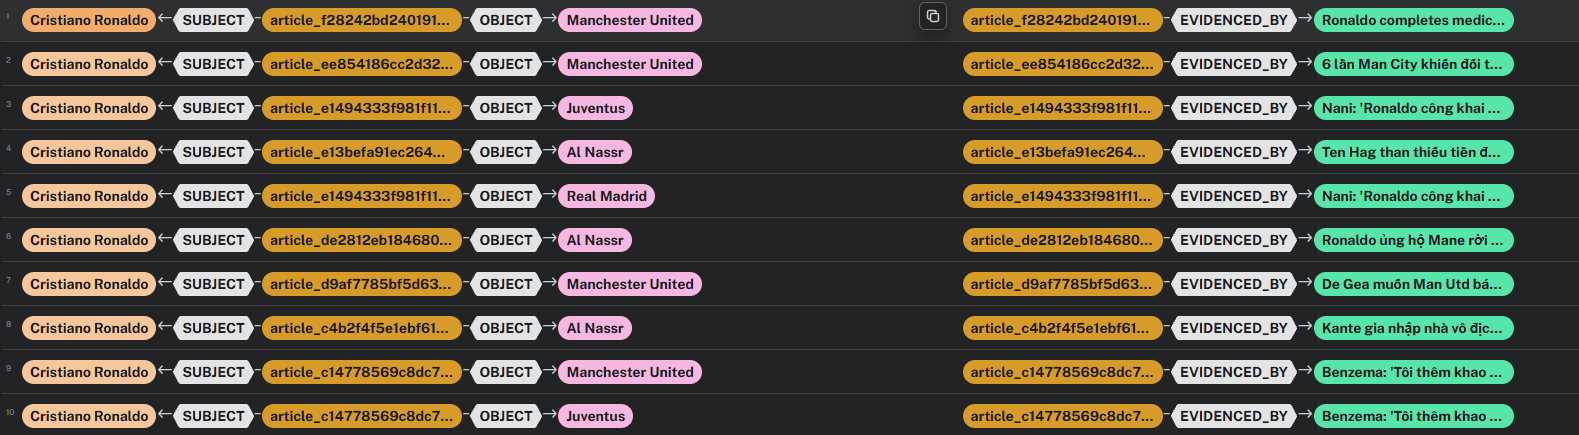
\includegraphics[width=0.49\linewidth,height=5.2cm,keepaspectratio]{figures/neo4j_evidence.png}}{\fbox{\parbox[c][4.5cm]{0.46\linewidth}{\centering evidence trace (Neo4j)}}}\hfill
\IfFileExists{figures/neo4j_path.png}{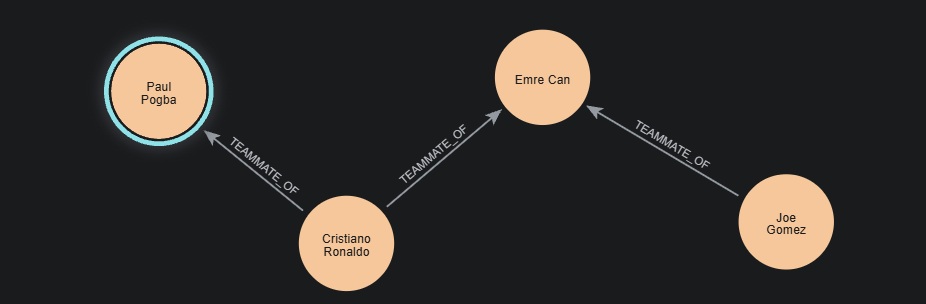
\includegraphics[width=0.49\linewidth,height=5.2cm,keepaspectratio]{figures/neo4j_path.png}}{\fbox{\parbox[c][4.5cm]{0.46\linewidth}{\centering shortest teammate path (Neo4j)}}}
\caption{Left: an extracted relation traced back to its evidence sentence and source article. Right: a shortest path in the teammate network.}
\label{fig:neo4j}
\end{figure}

% =====================================================================
\section{Graph Quality}
\subsection{Precision}
We graded a random sample of 150 edges of the 14B graph by hand, labelling each edge correct, wrong or unsure against its evidence and our knowledge of the facts. The 14B graph is 94.0\% correct (Wilson 95\% interval 89.0--96.8\%) when unsure edges count as wrong, and 97.2\% when they are left out.

The two graphs share 3,901 edges, which make up 79\% of the 4B graph; these edges are 97.1\% correct in the 14B sample. To estimate the precision of the 4B graph, we additionally graded 60 random edges that appear only in the 4B graph. 47 of them are correct (78.3\%, Wilson interval 66.4--86.9\%). Weighting the two parts by their size gives an estimated precision of 93.2\% for the 4B graph. Edges found only by the 14B model are more reliable (86.7\% in its sample). The difference between the two graphs is thus concentrated in the edges each model finds alone. % NOTE: the 60-edge 4B-only sample must be graded by both authors before submission.

\begin{table}[t]\centering\small
\caption{The 4B and 14B graphs. Precision of the 4B graph is estimated from shared and 4B-only edges.}
\label{tab:graphs}
\begin{tabular}{@{}lrr@{}}\toprule
& Qwen3-4B (final) & Qwen3-14B\\\midrule
Nodes / extracted edges & 2,046 / 4,924 & 2,147 / 5,111\\
Nodes with a Wikidata identifier & 97.8\% & 97.9\%\\
Edges with $\geq 2$ evidence sentences & 57.0\% & 56.9\%\\
Edges with evidence in both languages & 19.8\% & 19.9\%\\
Edges removed by the Wikidata filter & 1,795 & 980\\
Shared edges & \multicolumn{2}{c}{3,901 (Jaccard 0.64)}\\
Precision & $\approx$93.2\% (estimated) & 94.0\% (89.0--96.8)\\\bottomrule
\end{tabular}
\end{table}

\subsection{Error analysis}
The 13 wrong edges in the 4B-only sample fall into a few patterns:
\begin{itemize}
\item \textbf{The opponent's club (4).} ``Brentford beat Man Utd'' led to Brentford players being attached to Manchester United.
\item \textbf{Confused roles (3).} A goalkeeper ``managing'' his club, a club co-owner ``playing for'' it, and a former player under Guardiola ``managing'' Bayern Munich.
\item \textbf{Reversed transfers or loans (2).} ``West Ham sold Rice'' became a transfer to West Ham.
\item \textbf{Events that did not happen (1).} A player who ``almost joined'' a club.
\item \textbf{A wrongly linked person (1).} ``Pedro Mendes'' was written for the agent Jorge Mendes.
\item \textbf{Unrelated evidence (2).}
\end{itemize}
Three further edges are true facts, but their sentence states the opposite direction. Two of the patterns, reading the sentence in the wrong direction and confusing roles, reappear in question answering (Section~\ref{sec:qa}).

% =====================================================================
\section{Social Network Analysis}
\subsection{Extracted graph}
The extracted graph has density 0.0018 and average degree 3.6. Its largest connected component holds 2,039 of the 2,046 nodes. Club PageRank follows media attention: Manchester United (0.030), Chelsea (0.026), Arsenal (0.022), Liverpool (0.020), Tottenham Hotspur (0.019) and Manchester City (0.019). More than half of the edges (57\%) have at least two evidence sentences, and 974 edges have evidence in both languages.

\subsection{Small world}
We compare the average shortest path $L$ and the clustering coefficient $C$ of each network's largest component with the mean of 10 random $G(n,m)$ graphs that have the same number of nodes and edges:
\[\sigma = \frac{C/C_{r}}{L/L_{r}}.\]
A network is a small world when $\sigma > 1$. We also report an approximate $\omega = L_r/L - C/C_\ell$, using the clustering $C_\ell$ of a ring lattice with the same mean degree.

\begin{table}[t]\centering\small
\caption{Small-world test on the derived networks of the 4B graph ($r$: mean of 10 random graphs).}
\label{tab:smallworld}
\begin{tabular}{@{}lrrcccccc@{}}\toprule
Network & Nodes & Edges & $L$ & $L_r$ & $C$ & $C_r$ & $\sigma$ & $\omega$\\\midrule
Teammates & 1,433 & 41,258 & 2.438 & 2.054 & 0.441 & 0.040 & 9.23 & 0.244\\
Teammates + played under & 1,482 & 46,591 & 2.325 & 2.024 & 0.436 & 0.042 & 8.95 & 0.279\\
Transfer flow (clubs) & 194 & 2,169 & 2.162 & 1.949 & 0.456 & 0.116 & 3.55 & 0.264\\\bottomrule
\end{tabular}
\end{table}

All three networks are small worlds (Table~\ref{tab:smallworld}). Any two players are on average 2.4 teammate steps apart, while clustering is eleven times higher than in a random graph. Part of this clustering comes from the projection itself, since every squad forms a dense cluster.

\subsection{Centrality}
In the teammate network, the highest degrees belong to much-travelled players: Danny Welbeck (203 teammates), Romelu Lukaku (185), Victor Moses and Raheem Sterling (175). The same names lead PageRank. The highest sampled betweenness belongs to long careers that bridge generations and clubs: Mark Hughes, James Milner, Danny Welbeck and Mark Schwarzer. In the extracted graph, coaches and pundits stand out instead, because they appear in many criticism edges.

\subsection{Communities and nuclei}
\begin{table}[t]\centering\small
\caption{Community detection on the teammate network, and the nucleus (inner $k$-core) of the six largest Leiden communities.}
\label{tab:communities}
\begin{tabular}{@{}lccc@{}}\toprule
Algorithm & Communities & Modularity & NMI with main club\\\midrule
Leiden & 13 & 0.422 & 0.620\\
Louvain & 11 & 0.406 & 0.593\\
Label propagation & 7 & 0.001 & 0.027\\\bottomrule
\end{tabular}\\[0.6em]
\begin{tabular}{@{}rlcl@{}}\toprule
Size & Main club & Nucleus $k$ & Typical members\\\midrule
250 & Chelsea & 33 & César Azpilicueta, Romelu Lukaku, Victor Moses\\
198 & Manchester United (older squads) & 38 & Jonny Evans, Darren Fletcher, Ryan Giggs\\
152 & West Ham United & 16 & James Ward-Prowse, Cheikhou Kouyaté, Michail Antonio\\
142 & Manchester United (recent squads) & 35 & Casemiro, Luke Shaw, Raphaël Varane\\
128 & Tottenham Hotspur & 28 & Harry Kane, Ben Davies, Hugo Lloris\\
115 & Arsenal & 37 & Héctor Bellerín, Reiss Nelson, Ainsley Maitland-Niles\\\bottomrule
\end{tabular}
\end{table}

Leiden and Louvain reach a modularity of about 0.41--0.42, and their communities agree with each player's main club (NMI 0.62; Table~\ref{tab:communities}). Label propagation merges almost the whole network into one community, so it does not suit a network this dense. Interestingly, Manchester United splits into two communities, one for older and one for recent squads, because spells that do not overlap in time create no teammate edges.

The $k$-core decomposition \cite{seidman1983network} gives the nucleus of the network. The maximum core is $k=41$ and holds 563 people (density 0.117). Core number and degree are strongly correlated (Spearman 0.937), and all of the 20 highest-PageRank players lie in the main core. Inside each community, the innermost core identifies the squad that held the community together. Nuclei with a high $k$ (Manchester United 38, Arsenal 37) indicate long, stable squads. The low nucleus of the West Ham community ($k=16$) indicates a community held together by turnover rather than by one core squad.

\textbf{Robustness.} Every conclusion holds on the 14B graph: $\sigma=9.54$, $L=2.46$, $C=0.447$, Leiden modularity 0.434 with NMI 0.64, $k_{\max}=42$ with 562 people in the main core, and the same five leaders by PageRank. The smaller extraction model therefore changes individual edges but not the structure of the network.

% =====================================================================
\section{Multi-hop Question Answering}\label{sec:qa}
\begin{figure}[t]\centering
\resizebox{\linewidth}{!}{\begin{tikzpicture}[font=\scriptsize,node distance=0.32cm and 0.4cm,
 b/.style={draw,rounded corners=2pt,align=center,text width=2.05cm,minimum height=0.85cm,fill=#1!8},
 arr/.style={-{Stealth},thick}]
\node[b=gray](q){Question};
\node[b=blue,right=of q](l){Entity linking\\ \tiny names, surnames, prominence};
\node[b=blue,right=of l](r){Router};
\node[b=orange,above right=0.15cm and 0.4cm of r](t){Analytics tools\\ \tiny PageRank, k-core, nucleus, path};
\node[b=orange,below right=0.15cm and 0.4cm of r](p){Fast planner\\ \tiny 1 call, JSON schema};
\node[b=green,right=of p](v){Checks V0--V5\\ \tiny deterministic};
\node[b=red,below=of v](th){Re-plan with\\ reasoning \tiny(streamed)};
\node[b=green,right=of v](c){Compile Cypher\\ \tiny read-only};
\node[b=gray,right=of c](a){Answer + evidence\\ \tiny + subgraph};
\draw[arr](q)--(l);\draw[arr](l)--(r);\draw[arr](r)|-(t);\draw[arr](r)|-(p);\draw[arr](p)--(v);
\draw[arr](v)--node[above,font=\tiny]{pass}(c);\draw[arr](v)--node[right,font=\tiny]{flag}(th);\draw[arr](th)-|(c);
\draw[arr](c)--(a);\draw[arr](t)-|(a);
\end{tikzpicture}}
\caption{Question answering. The model chooses hops; code type-checks them, runs deterministic checks, compiles the plan to Cypher and renders the answer with its evidence. Reasoning is used only for flagged plans.}
\label{fig:qa}
\end{figure}

\subsection{From questions to plans}
Writing Cypher directly is hard for a small model: it must recall the schema, relation directions and syntax at the same time. Instead, the model writes a plan over a catalogue of 29 named, typed hops. Each hop has an input type, an output type and a direction; for example \hop{coaches_of_player} follows \rel{PLAYED_UNDER} outward from a person, and \hop{players_of_club} follows \rel{PLAYS_FOR} inward from a club. A plan has one chain, or two chains whose results are intersected, with at most three hops each, and an output of \texttt{list} or \texttt{count}. For example, ``\vi{Các HLV từng huấn luyện Bukayo Saka đã dẫn dắt những CLB nào?}'' (Which clubs have the coaches of Bukayo Saka managed?) becomes:
\begin{center}\footnotesize\texttt{\{"chains":[\{"from":"person","hops":["coaches\_of\_player","clubs\_managed"]\}],"output":"list"\}}\end{center}
Code type-checks the plan, compiles it to a single read-only Cypher query, and computes how many entities each hop reaches. These counts appear in the interface as the steps of the reasoning. Decoding is constrained by a JSON schema whose enumerations contain only the hop names and the parameters found by the linker. Eight examples are retrieved from a library of 52 by word overlap and parameter types. Entities are linked by exact names and aliases, by capitalised surnames, and by prominence: a bare surname resolves to a person who has at least three times as many graph links as the runner-up (``Kane'' resolves to Harry Kane), and is otherwise reported as ambiguous with suggestions. Questions about the whole network go to analytics tools instead: PageRank, the network nucleus, a person's community nucleus and the shortest teammate path between two people.

\subsection{Deterministic checks and escalation}
The first plan comes from a single greedy call. Six checks then run without any model call:
\begin{itemize}
\item \textbf{V0}: every hop's input type matches the current entity type;
\item \textbf{V1}: every entity found by the linker is used;
\item \textbf{V2}: each hop's input has the expected role (\hop{players_coached} expects a coach, \hop{coaches_of_player} a player). Roles combine labels with roles proven by edges, because labels alone are incomplete;
\item \textbf{V3}: every relation cue word in the question (``\vi{đồng đội}'' teammate, ``\vi{học trò}'' pupil, ``\vi{khoác áo}'' played for, \dots) is covered by a hop of that relation;
\item \textbf{V4}: the plan returns rows unless the question asks whether something exists;
\item \textbf{V5}: the answer type asked for (``which club'', ``who'', ``how many'') matches the plan's output.
\end{itemize}
If a check fires, the model re-plans once with reasoning enabled, receiving the problems as feedback. The new plan replaces the fast plan only if it raises strictly fewer problems. Reasoning calls are streamed, because the tunnel used for serving cuts responses that start after 100\,s.

\subsection{Answers, interface and serving}
Answer rows are rendered by code, never written by the model. Each row of a single-hop news relation cites its own evidence sentence and article; derived results are explained by the drawn path. The Streamlit interface has three pages:
\begin{itemize}
\item a \emph{network overview}: small world, communities, $k$-core nuclei and central people;
\item a \emph{node portrait}: degree, PageRank and core number with their ranks, the person's community and its nucleus, an interactive ego network, the extracted relations and the latest evidence sentences;
\item \emph{multi-hop question answering}: the linked entities, the route, each hop with its count, the checks, the Cypher query, the cited answer and the explaining subgraph.
\end{itemize}
Qwen3-4B is served by vLLM on two Kaggle T4 GPUs (fp16, tensor parallelism 2), exposed through a tunnel whose address is discovered automatically.

\begin{figure}[t]\centering
\IfFileExists{figures/app_portrait.png}{\includegraphics[width=0.49\linewidth]{figures/app_portrait.png}}{\fbox{\parbox[c][4.2cm]{0.46\linewidth}{\centering node portrait (screenshot)}}}\hfill
\IfFileExists{figures/app_qa.png}{\includegraphics[width=0.49\linewidth]{figures/app_qa.png}}{\fbox{\parbox[c][4.2cm]{0.46\linewidth}{\centering question answering with trace (screenshot)}}}
\caption{The application. Left: portrait of a node with its network position and ego network. Right: a multi-hop answer with the reasoning steps, automatic checks, evidence and explaining subgraph.}
\label{fig:app}
\end{figure}

% =====================================================================
\section{Experiments}
\subsection{Benchmarks}
Answers are scored by execution accuracy: the returned rows must exactly match those of a reference query on the fixed graph. Canonical entity parameters are supplied, so entity linking is not scored, and reference queries are never shown to the model. We use three benchmarks:
\begin{itemize}
\item \textbf{v1}: 32 hand-written questions (8 development, 24 test).
\item \textbf{v2}: 100 generated questions: 30 lookups, 35 multi-hop (10 of them three-hop), 15 counts, 15 intersections and 5 with an empty answer. The errors on v2 were inspected, so it serves as the development set.
\item \textbf{v2b}: a held-out set of 100 questions built with the same generator from 102 entities that appear neither in v2 nor in the example library. The final system was run on it once.
\end{itemize}
All runs use Qwen3-4B without fine-tuning.

\subsection{Results}
\begin{table}[t]\centering\small
\caption{Text2Cypher against hop planning on the 24 v1 test questions (Qwen3-4B).}
\label{tab:v1}
\begin{tabular}{@{}lcc@{}}\toprule
Method & Correct & Mean time\\\midrule
Text2Cypher, schema only & 6 / 24 & --\\
Text2Cypher, few-shot & 12 / 24 & --\\
Text2Cypher, few-shot + reasoning & 14 / 24 & 25.4\,s\\
Hop planner, one call & 21 / 24 & 2.0\,s\\
Hop planner + reasoning & 23 / 24 & 23.8\,s\\\bottomrule
\end{tabular}
\end{table}

\begin{table}[t]\centering\small
\caption{Planner variants on the development (v2) and held-out (v2b) sets. Time is the mean (median) seconds per question.}
\label{tab:ablation}
\begin{tabular}{@{}lcccc@{}}\toprule
& \multicolumn{2}{c}{v2 (dev)} & \multicolumn{2}{c}{v2b (held-out)}\\\cmidrule(lr){2-3}\cmidrule(lr){4-5}
Variant & Correct & Time & Correct & Time\\\midrule
One call, 20 fixed examples & 78 & 2.3 & 73 & 2.0\\
+ JSON schema, retrieved examples & 81 & 2.7 & -- & --\\
+ 3-vote self-consistency, reasoning on ties & 86 & 4.6 & 89 & 2.8\\
\quad + role labels in the prompt & 83 & 3.7 & 88 & 4.1\\
Always reasoning & 92 & 30.6 & 94 & 28.6\\
\textbf{Fast plan + checks + selective reasoning} & \textbf{98} & 9.9 (1.7) & \textbf{95} & 6.7 (1.8)\\
\quad fast plan alone (no escalation) & 82 & -- & 84 & --\\\bottomrule
\end{tabular}
\end{table}

\textbf{Planning beats query writing.} On the same 24 questions, a single planning call answers 21, while Text2Cypher with examples answers 12 (Table~\ref{tab:v1}). Constraining the output to typed hops removes most of the ways a small model can go wrong.

\textbf{Voting does not help.} On v2b, taking only the greedy vote and escalating it when it is invalid gives exactly the same score as three-vote self-consistency. No majority ever overturned the greedy plan, and 21 of the 22 wrong answers were unanimous. The planner's errors are systematic: sampling repeats the same misreading of a phrase. The apparent gain of voting comes entirely from re-planning invalid plans with reasoning.

\textbf{Knowledge belongs in checks, not prompts.} Adding role labels to the prompt fixed the direction of coach--player questions, but it broke others, for instance by reversing a question about a person who was both player and coach. Overall it lowered accuracy by 1--3 points. The same knowledge used as a check (V2) fixes those questions without side effects.

\textbf{Selective reasoning.} Always-on reasoning is accurate (94\%) but slow (28.6\,s, 90th percentile 48\,s), and it makes its own errors. For example, it confuses the aggregate club-to-club transfer flow with individual transfers, and it shortens ``coaches of the players of a club'' to ``coaches of the club''. The fast planner gets most of those questions right. Escalating only the 17--21\% of plans that fail a check combines the strengths of both: 98\% on the development set and 95\% on the held-out set. Escalation repaired 11--16 plans and broke none, and the median time per question stays below 2\,s. On the final 4B graph, the held-out accuracy is 96\%.

\textbf{Remaining errors.} On the held-out set, the final system still fails five questions. Two are existence questions answered with a count of zero instead of an empty list; the meaning is the same, so a lenient score would give 97\%. Two read ``who criticised X'' in the wrong direction; no check can catch this, since both directions return rows. The last one chooses ``appointed by'' instead of ``managed''.

\subsection{Limitations}
The v2 and v2b benchmarks come from the same phrasing templates, so v2b is held out in entities but not in phrasing. Because the checks were designed from errors on v2, the scores on generated questions are optimistic. A benchmark written by people, evaluated end to end including entity linking, is needed for a realistic estimate. Graph precision is estimated from samples graded by the authors, without an independent annotator. Derived networks depend on the completeness of career dates in Wikidata.

% =====================================================================
\section{Conclusion}
We built a bilingual, evidence-backed Premier League social network of 2,046 nodes and 4,924 edges, with a 4B model doing all of the language work. Distillation and a Wikidata confirmation filter keep graph precision within about a point of a 14B model. The derived networks are small worlds whose communities and $k$-core nuclei follow squads, and these conclusions do not depend on which model extracted the graph. For question answering, a small model plans much better than it writes queries. Its remaining mistakes are systematic, so deterministic checks with selective reasoning work where self-consistency voting does not, reaching 95\% on held-out questions at interactive speed. Future work includes a human-written, end-to-end benchmark, independent annotation of graph quality, and checks for relation direction that do not rely on roles.

\section*{Data and Code Availability}
Code, the graph (nodes, edges, source-article links, derived networks), network-analysis results, graded samples and benchmarks are available at \url{https://github.com/minquanle/premier-league-graph}. Article texts and evidence sentences are not redistributed, for copyright reasons. Every edge links to its source articles.

\begingroup\small
\begin{thebibliography}{99}\setlength{\itemsep}{1pt}
\bibitem{pan2024unifying} S.~Pan, L.~Luo, Y.~Wang, C.~Chen, J.~Wang, X.~Wu. Unifying large language models and knowledge graphs: A roadmap. \textit{IEEE Transactions on Knowledge and Data Engineering}, 36(7):3580--3599, 2024.
\bibitem{zhou2024universalner} W.~Zhou, S.~Zhang, Y.~Gu, M.~Chen, H.~Poon. UniversalNER: Targeted distillation from large language models for open named entity recognition. In \textit{ICLR}, 2024.
\bibitem{hinton2015distilling} G.~Hinton, O.~Vinyals, J.~Dean. Distilling the knowledge in a neural network. \textit{arXiv:1503.02531}, 2015.
\bibitem{hu2022lora} E.~J.~Hu, Y.~Shen, P.~Wallis, Z.~Allen-Zhu, Y.~Li, S.~Wang, L.~Wang, W.~Chen. LoRA: Low-rank adaptation of large language models. In \textit{ICLR}, 2022.
\bibitem{yang2025qwen3} A.~Yang et al. Qwen3 technical report. \textit{arXiv:2505.09388}, 2025.
\bibitem{kwon2023efficient} W.~Kwon, Z.~Li, S.~Zhuang, Y.~Sheng, L.~Zheng, C.~H.~Yu, J.~Gonzalez, H.~Zhang, I.~Stoica. Efficient memory management for large language model serving with PagedAttention. In \textit{SOSP}, 2023.
\bibitem{vrandecic2014wikidata} D.~Vrande\v{c}i\'{c}, M.~Kr\"{o}tzsch. Wikidata: A free collaborative knowledgebase. \textit{Communications of the ACM}, 57(10):78--85, 2014.
\bibitem{watts1998collective} D.~J.~Watts, S.~H.~Strogatz. Collective dynamics of `small-world' networks. \textit{Nature}, 393:440--442, 1998.
\bibitem{humphries2008network} M.~D.~Humphries, K.~Gurney. Network `small-world-ness': A quantitative method for determining canonical network equivalence. \textit{PLoS ONE}, 3(4):e0002051, 2008.
\bibitem{telesford2011ubiquity} Q.~K.~Telesford, K.~E.~Joyce, S.~Hayasaka, J.~H.~Burdette, P.~J.~Laurienti. The ubiquity of small-world networks. \textit{Brain Connectivity}, 1(5):367--375, 2011.
\bibitem{page1999pagerank} L.~Page, S.~Brin, R.~Motwani, T.~Winograd. The PageRank citation ranking: Bringing order to the web. Technical report, Stanford InfoLab, 1999.
\bibitem{blondel2008fast} V.~D.~Blondel, J.-L.~Guillaume, R.~Lambiotte, E.~Lefebvre. Fast unfolding of communities in large networks. \textit{Journal of Statistical Mechanics}, P10008, 2008.
\bibitem{traag2019louvain} V.~A.~Traag, L.~Waltman, N.~J.~van~Eck. From Louvain to Leiden: Guaranteeing well-connected communities. \textit{Scientific Reports}, 9:5233, 2019.
\bibitem{raghavan2007near} U.~N.~Raghavan, R.~Albert, S.~Kumara. Near linear time algorithm to detect community structures in large-scale networks. \textit{Physical Review E}, 76:036106, 2007.
\bibitem{newman2006modularity} M.~E.~J.~Newman. Modularity and community structure in networks. \textit{PNAS}, 103(23):8577--8582, 2006.
\bibitem{seidman1983network} S.~B.~Seidman. Network structure and minimum degree. \textit{Social Networks}, 5(3):269--287, 1983.
\bibitem{batagelj2003m} V.~Batagelj, M.~Zaver\v{s}nik. An $O(m)$ algorithm for cores decomposition of networks. \textit{arXiv:cs/0310049}, 2003.
\bibitem{lewis2020retrieval} P.~Lewis et al. Retrieval-augmented generation for knowledge-intensive NLP tasks. In \textit{NeurIPS}, 2020.
\bibitem{edge2024local} D.~Edge, H.~Trinh, N.~Cheng, J.~Bradley, A.~Chao, A.~Mody, S.~Truitt, J.~Larson. From local to global: A graph RAG approach to query-focused summarization. \textit{arXiv:2404.16130}, 2024.
\bibitem{ozsoy2024text2cypher} M.~G.~Ozsoy, L.~Messallem, J.~Besga, G.~Minneci. Text2Cypher: Bridging natural language and graph databases. \textit{arXiv:2412.10064}, 2024.
\bibitem{wang2023selfconsistency} X.~Wang, J.~Wei, D.~Schuurmans, Q.~Le, E.~Chi, S.~Narang, A.~Chowdhery, D.~Zhou. Self-consistency improves chain of thought reasoning in language models. In \textit{ICLR}, 2023.
\bibitem{chen2024teaching} X.~Chen, M.~Lin, N.~Sch\"{a}rli, D.~Zhou. Teaching large language models to self-debug. In \textit{ICLR}, 2024.
\bibitem{ni2023lever} A.~Ni, S.~Iyer, D.~Radev, V.~Stoyanov, W.~Yih, S.~Wang, X.~V.~Lin. LEVER: Learning to verify language-to-code generation with execution. In \textit{ICML}, 2023.
\bibitem{zhang2023coder} T.~Zhang, T.~Yu, T.~Hashimoto, M.~Lewis, W.~Yih, D.~Fried, S.~Wang. Coder reviewer reranking for code generation. In \textit{ICML}, 2023.
\end{thebibliography}
\endgroup
\end{document}
